\begin{figure}[h!]
    \caption{Vigencias futuras e inversión pública (\% PIB)}
    \label{fig:VF}
    \centering
    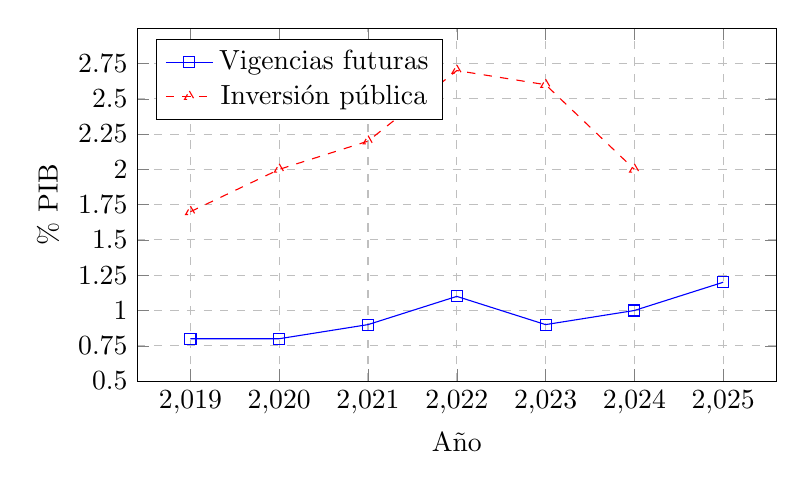
\begin{tikzpicture}
        \begin{axis}[
            width=0.8\textwidth,
            height=0.5\textwidth,
            grid=major,
            xlabel={Año},
            ylabel={\% PIB},
            ymin=0.5, ymax=3.0,
            xtick={2019, 2020, 2021, 2022, 2023, 2024, 2025},
            %ytick={0.5, 1.0, 1.5, 2.0, 2.5},
            ytick={0.50, 0.75, 1.00, 1.25, 1.50, 1.75, 2.00, 2.25, 2.50,2.75},
            legend pos=north west,
            ymajorgrids=true,
            xmajorgrids=true,
            grid style=dashed,
        ]
        \addplot[
            color=blue,
            mark=square,
        ]
        coordinates {
            (2019,0.8)
            (2020,0.8)
            (2021,0.9)
            (2022,1.1)
            (2023,0.9)
            (2024,1.0)
            (2025,1.2)
        };

        \addplot[
            color=red,
            mark=triangle, dashed
        ]
        coordinates {
            (2019,1.7)
            (2020,2.0)
            (2021,2.2)
            (2022,2.7)
            (2023,2.6)
            (2024,2.0)
        };
        \legend{Vigencias futuras, Inversión pública}
        \end{axis}
    \end{tikzpicture}
\vspace{0.3cm}
\par\footnotesize{\textit{Fuente: Elaboración propia con base en Marcos Fiscales de Mediano Plazo 2018--2024 y Balance del GNC, Ministerio de Hacienda.}}
\end{figure}

\begin{comment}
\begin{figure}[h!]
    \caption{Vigencias futuras para inversión (\% PIB)}
    \label{fig:VF}
    \centering
    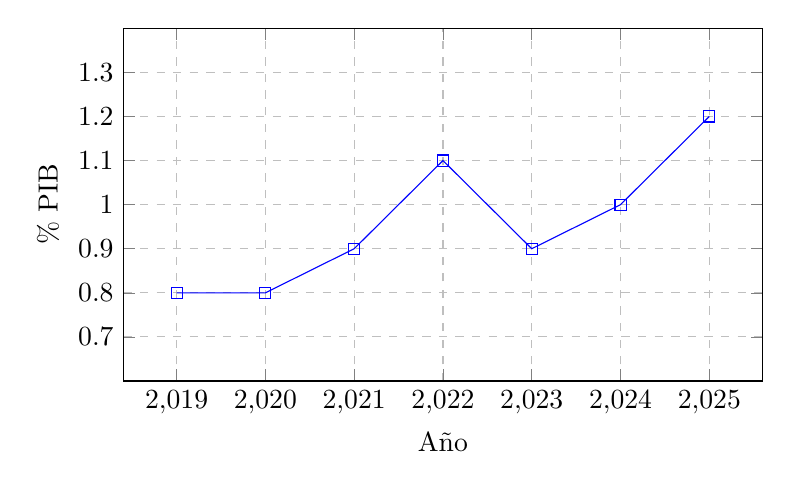
\begin{tikzpicture}
        \begin{axis}[
            width=0.8\textwidth,
            height=0.5\textwidth,
            grid=major,
            xlabel={Año},
            ylabel={\% PIB},
            ymin=0.6, ymax=1.4,
            xtick={2019, 2020, 2021, 2022, 2023,2024,2025},
            ytick={0.7, 0.8, 0.9, 1.0, 1.1, 1.2, 1.3},
            legend pos=north west,
            ymajorgrids=true,
            xmajorgrids=true,
            grid style=dashed,
        ]
        \addplot[
            color=blue,
            mark=square,
            ]
            coordinates {
            (2019,0.8)
            (2020,0.8)
            (2021,0.9)
            (2022,1.1)
            (2023,0.9)
            (2024,1.0)
            (2025,1.2)
            };
        %\legend{VF (\% PIB)}
        \end{axis}
    \end{tikzpicture}
\vspace{0.3cm}
\par\footnotesize{\textit{Fuente: Elaboración propia con base en Marcos Fiscales de Mediano Plazo 2018-2024, Ministerio de Hacienda.}}
\end{figure}
\end{comment}